\documentclass[border=5mm]{standalone}
\usepackage{tikz}
\usetikzlibrary{calc}           % For general calculations
\usetikzlibrary{matrix}         % For the matrix cmd
\usetikzlibrary{positioning}    % For above = Xcm of and similars
\usetikzlibrary{intersections}  % Mainly here for the arc over line
\usetikzlibrary{topaths}        % Enable move to operation
\usetikzlibrary{backgrounds}    % Put colors in background

%%% Sourced from https://tex.stackexchange.com/questions/241357/wiring-diagrams-with-pinout
%%% Adapted from https://tex.stackexchange.com/a/111674/114143
%%% provides syntax for jumping lines
\tikzset{
    connect/.style args={(#1) to (#2) over #3 by #4}{
        insert path={
            \pgfextra{
                \pgfinterruptpath
                    \path [name path=userpath] (#1) -- (#2);
                    \path [name intersections={of=userpath and #3,by=overpoint}];
                \endpgfinterruptpath                
            }
            let \p1=($(#1)-(overpoint)$), \n1={veclen(\x1,\y1)}, 
                            \n2={atan2(\y1,\x1)}, \n3={abs(#4)}, \n4={#4>0 ?180:-180}  in 
                            (#1) -- ($(#1)!\n1-\n3!(overpoint)$) 
                            arc (\n2:\n2+\n4:\n3) -- (#2)
        }
    },
}

%% Block styles (to avoid repetition and ease our lives)
\tikzset{wire board/.style={matrix of nodes,
                            row sep=2mm,
                            nodes={anchor=center}
                            },
        jetson/.style={column 1/.style={nodes={left}},
                                       column 3/.style={nodes={above right}},
                                       column 2/.style={font=\bfseries}
                                       },
        gps/.style={column 1/.style={nodes={above left}},
                                       column 3/.style={nodes={right}},
                                       column 2/.style={font=\bfseries}
                                       },
        lidar/.style={column 1/.style={nodes={above left}},
                                       column 3/.style={nodes={right}},
                                       column 2/.style={font=\bfseries}
                                       },
        camera/.style={column 1/.style={nodes={above left}},
                                       column 3/.style={nodes={right}},
                                       column 2/.style={font=\bfseries}
                                       },
        wifi/.style={column 1/.style={nodes={above left}},
                                       column 3/.style={nodes={right}},
                                       column 2/.style={font=\bfseries}
                                       },
        controller/.style={column 1/.style={nodes={above left}},
                                       column 3/.style={nodes={right}},
                                       column 2/.style={font=\bfseries}
                                       },
        vesc/.style={column 1/.style={nodes={left}},
                                       column 3/.style={nodes={above right}},
                                       column 2/.style={font=\bfseries}
                                       },
        pdbL/.style={column 1/.style={nodes={above left}},
                                       column 3/.style={nodes={right}},
                                       column 2/.style={font=\bfseries}
                                       },
        pdbR/.style={column 1/.style={nodes={left}},
                                       column 3/.style={nodes={above right}},
                                       column 2/.style={font=\bfseries}
                                       },
        bldc/.style={column 1/.style={nodes={above left}},
                                       column 3/.style={nodes={right}},
                                       column 2/.style={font=\bfseries}
                                       },
        dc2dc/.style={column 1/.style={nodes={left}},
                                       column 3/.style={nodes={above right}},
                                       column 2/.style={font=\bfseries}
                                       },
        splitterL/.style={column 1/.style={nodes={above left}},
                                       column 3/.style={nodes={right}},
                                       column 2/.style={font=\bfseries}
                                       },
        splitterR/.style={column 1/.style={nodes={left}},
                                       column 3/.style={nodes={above right}},
                                       column 2/.style={font=\bfseries}
                                       },
        antisparkL/.style={column 1/.style={nodes={above left}},
                                       column 3/.style={nodes={right}},
                                       column 2/.style={font=\bfseries}
                                       },
        antisparkR/.style={column 1/.style={nodes={left}},
                                       column 3/.style={nodes={above right}},
                                       column 2/.style={font=\bfseries}
                                       },
        servo/.style={column 1/.style={nodes={above left}},
                                       column 3/.style={nodes={right}},
                                       column 2/.style={font=\bfseries}
                                       },
        battery/.style={column 1/.style={nodes={above left}},
                                       column 3/.style={nodes={right}},
                                       column 2/.style={font=\bfseries}
                                       },
        power/.style={column 1/.style={nodes={above left}},
                                       column 3/.style={nodes={right}},
                                       column 2/.style={font=\bfseries}
                                       },
}

%% Colors
\definecolor{beaublue}{rgb}{0.86, 0.9, 0.93}
\definecolor{usbblue}{rgb}{0.19, 0.55, 0.91}



\begin{document}
\sffamily
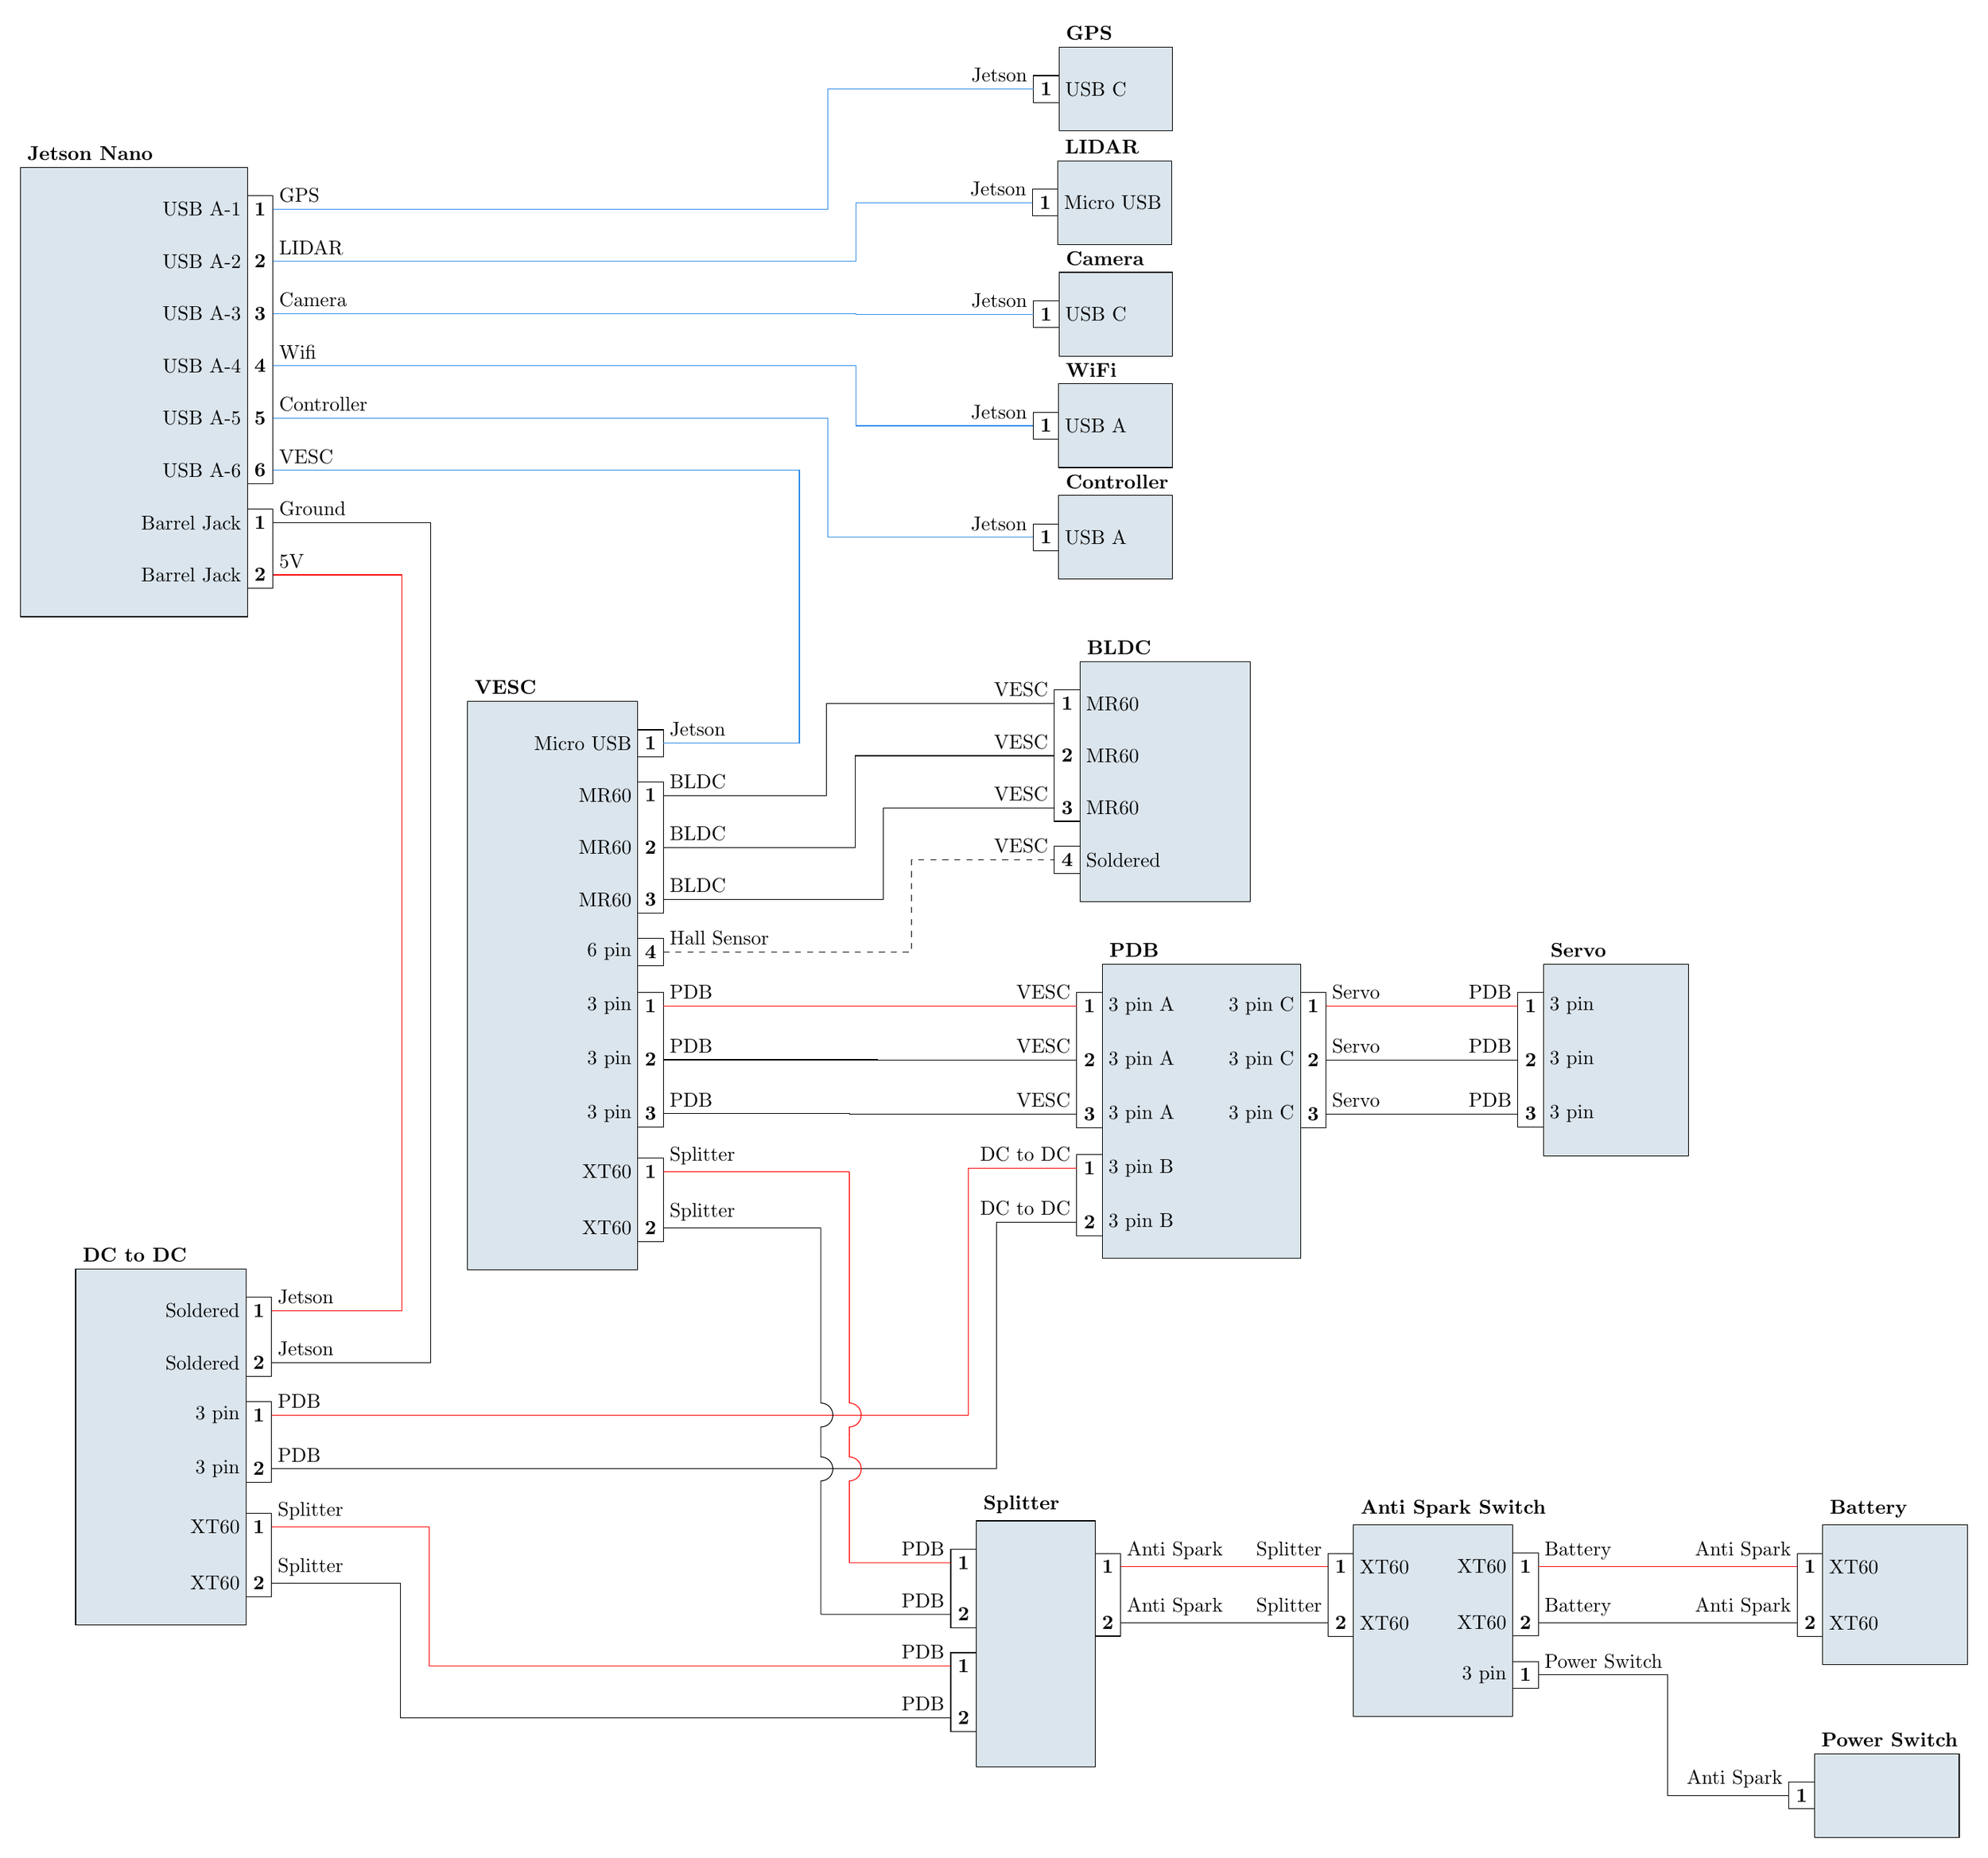
\begin{tikzpicture}
%% Drawing the first block (jetson)
    \matrix[wire board,jetson] (jetson) {
        USB A-1     &   1   &   GPS         \\
        USB A-2     &   2   &   LIDAR       \\
        USB A-3     &   3   &   Camera      \\
        USB A-4     &   4   &   Wifi        \\
        USB A-5     &   5   &   Controller  \\
        USB A-6     &   6   &   VESC        \\
        Barrel Jack &   1   &   Ground      \\
        Barrel Jack &   2   &   5V          \\
    };
    \draw (jetson-1-2.north east) rectangle (jetson-6-2.south west); % USB
    \draw (jetson-7-2.north east) rectangle (jetson-8-2.south west); % Barrel Jack
    \scoped[on background layer]{\draw [fill=beaublue] (jetson-1-2.north west)+(-4cm,0.5cm) node[above right, font=\bfseries]{Jetson Nano} rectangle ($(jetson-8-2.south west)+(0,-0.5cm)$);}

%% GPS
    \matrix[wire board, gps, matrix anchor=south, above right=1.151cm and 14cm of jetson.north] (gps) {
        Jetson  &   1   &   USB C \\
    };
    \draw (gps-1-2.north east) rectangle (gps-1-2.south west); % USB
    \scoped[on background layer]{\draw [fill=beaublue] (gps-1-2.north east)+(0cm,0.5cm) node[above right, align=center, font=\bfseries]{GPS} rectangle ($(gps-1-2.south east)+(2cm,-0.5cm)$);}

%% LIDAR
    \matrix[wire board, lidar, matrix anchor=south, below right=2cm and 0.3cm of gps.south] (lidar) {
        Jetson  &   1   &   Micro USB \\
    };
    \draw (lidar-1-2.north east) rectangle (lidar-1-2.south west); % USB
    \scoped[on background layer]{\draw [fill=beaublue] (lidar-1-2.north east)+(0cm,0.5cm) node[above right, align=center, font=\bfseries]{LIDAR} rectangle ($(lidar-1-2.south east)+(2cm,-0.5cm)$);}

%% Camera
    \matrix[wire board, camera, matrix anchor=north, below left=1cm and 0.3cm of lidar.south] (camera) {
        Jetson  &   1   &   USB C \\
    };
    \draw (camera-1-2.north east) rectangle (camera-1-2.south west); % USB
    \scoped[on background layer]{\draw [fill=beaublue] (camera-1-2.north east)+(0cm,0.5cm) node[above right, align=center, font=\bfseries]{Camera} rectangle ($(camera-1-2.south east)+(2cm,-0.5cm)$);}

%% Wifi
    \matrix[wire board, wifi, matrix anchor=north, below=1cm of camera.south] (wifi) {
        Jetson  &   1   &   USB A \\
    };
    \draw (wifi-1-2.north east) rectangle (wifi-1-2.south west); % USB
    \scoped[on background layer]{\draw [fill=beaublue] (wifi-1-2.north east)+(0cm,0.5cm) node[above right, align=center, font=\bfseries]{WiFi} rectangle ($(wifi-1-2.south east)+(2cm,-0.5cm)$);}

%% Controller
    \matrix[wire board, controller, matrix anchor=north, below=1cm of wifi.south] (controller) {
        Jetson  &   1   &   USB A \\
    };
    \draw (controller-1-2.north east) rectangle (controller-1-2.south west); % USB
    \scoped[on background layer]{\draw [fill=beaublue] (controller-1-2.north east)+(0cm,0.5cm) node[above right, align=center, font=\bfseries]{Controller} rectangle ($(controller-1-2.south east)+(2cm,-0.5cm)$);}

%% VESC
    \matrix[wire board, vesc, matrix anchor=north, below right=2cm and 7cm of jetson.south] (vesc) {
        Micro USB   &   1   &   Jetson      \\
        MR60        &   1   &   BLDC        \\
        MR60        &   2   &   BLDC        \\
        MR60        &   3   &   BLDC        \\
        6 pin       &   4   &   Hall Sensor \\
        3 pin       &   1   &   PDB         \\
        3 pin       &   2   &   PDB         \\
        3 pin       &   3   &   PDB         \\
        XT60        &   1   &   Splitter    \\
        XT60        &   2   &   Splitter    \\
    };
    \draw (vesc-1-2.north east) rectangle (vesc-1-2.south west); % USB
    \draw (vesc-2-2.north east) rectangle (vesc-4-2.south west); % BLDC
    \draw (vesc-5-2.north east) rectangle (vesc-5-2.south west); % Hall Sensor
    \draw (vesc-6-2.north east) rectangle (vesc-8-2.south west); % PDB
    \draw (vesc-9-2.north east) rectangle (vesc-10-2.south west); % splitterL
    \scoped[on background layer]{\draw [fill=beaublue] (vesc-1-2.north west)+(-3cm,0.5cm) node[above right, align=center, font=\bfseries]{VESC} rectangle ($(vesc-10-2.south west)+(0cm,-0.5cm)$);}

%% BLDC
    \matrix[wire board, bldc, matrix anchor=north, above right=.7cm and 7.5cm of vesc.north] (bldc) {
        VESC  &   1   & MR60        \\
        VESC  &   2   & MR60        \\
        VESC  &   3   & MR60        \\
        VESC  &   4   & Soldered    \\
    };
    \draw (bldc-1-2.north east) rectangle (bldc-3-2.south west); % VESC
    \draw (bldc-4-2.north east) rectangle (bldc-4-2.south west); % Hall Sensor
    \scoped[on background layer]{\draw [fill=beaublue] (bldc-1-2.north east)+(0cm,0.5cm) node[above right, align=center, font=\bfseries]{BLDC} rectangle ($(bldc-4-2.south east)+(3cm,-0.5cm)$);}

%% PDB
    \matrix[wire board, pdbL, matrix anchor=north, below=1.6069cm of bldc.south] (pdbL) {
        VESC        &   1   &   3 pin A \\
        VESC        &   2   &   3 pin A \\
        VESC        &   3   &   3 pin A \\
        DC to DC    &   1   &   3 pin B \\
        DC to DC    &   2   &   3 pin B \\
    };
    \matrix[wire board, pdbR, matrix anchor=north, right=4cm of pdbL.north] (pdbR) {
        3 pin C &   1   &   Servo   \\
        3 pin C &   2   &   Servo   \\
        3 pin C &   3   &   Servo   \\
    };
    \draw (pdbL-1-2.north east) rectangle (pdbL-3-2.south west); % VESC
    \draw (pdbL-4-2.north east) rectangle (pdbL-5-2.south west); % DC to DC
    \draw (pdbR-1-2.north east) rectangle (pdbR-3-2.south west); % Servo
    \scoped[on background layer]{\draw [fill=beaublue] (pdbL-1-2.north east)+(0cm,0.5cm) node[above right, align=center, font=\bfseries]{PDB} rectangle ($(pdbR-3-2.south west)+(0cm,-2.3cm)$);}

%% Servo
    \matrix[wire board, servo, matrix anchor=north, right=4cm of pdbR.north] (servo) {
        PDB     &   1   &   3 pin   \\
        PDB     &   2   &   3 pin   \\
        PDB     &   3   &   3 pin   \\
    };
    \draw (servo-1-2.north east) rectangle (servo-3-2.south west); % PDB
    \scoped[on background layer]{\draw [fill=beaublue] (servo-1-2.north east)+(0cm,0.5cm) node[above right, align=center, font=\bfseries]{Servo} rectangle ($(servo-3-2.south west)+(3cm,-0.5cm)$);}

%% DC to DC
    \matrix[wire board, dc2dc, matrix anchor=north, below=12cm of jetson.south] (dc2dc) {
        Soldered    &   1   &   Jetson      \\
        Soldered    &   2   &   Jetson      \\
        3 pin       &   1   &   PDB         \\
        3 pin       &   2   &   PDB         \\
        XT60        &   1   &   Splitter    \\
        XT60        &   2   &   Splitter    \\
    };
    \draw (dc2dc-1-2.north east) rectangle (dc2dc-2-2.south west); % Jetson
    \draw (dc2dc-3-2.north east) rectangle (dc2dc-4-2.south west); % splitterL
    \draw (dc2dc-5-2.north east) rectangle (dc2dc-6-2.south west); % PDB
    \scoped[on background layer]{\draw [fill=beaublue] (dc2dc-1-2.north west)+(-3cm,0.5cm) node[above right, align=center, font=\bfseries]{DC to DC} rectangle ($(dc2dc-6-2.south west)+(0cm,-0.5cm)$);}

%% Splitter
    \matrix[wire board, splitterL, matrix anchor=north, below left=5cm and 2.5cm of pdbL.south] (splitterL) {
        PDB     &   1   &   \\
        PDB     &   2   &   \\
        PDB     &   1   &   \\
        PDB     &   2   &   \\
    };
    \matrix[wire board, splitterR, matrix anchor=north, right=4cm of splitterL.north] (splitterR) {
                &   1   &   Anti Spark  \\
                &   2   &   Anti Spark  \\
    };
    \draw (splitterL-1-2.north east) rectangle (splitterL-2-2.south west); % VESC
    \draw (splitterL-3-2.north east) rectangle (splitterL-4-2.south west); % DC to DC
    \draw (splitterR-1-2.north east) rectangle (splitterR-2-2.south west); % Anti Spark
    \scoped[on background layer]{\draw [fill=beaublue] (splitterL-1-2.north east)+(0cm,0.5cm) node[above right, align=center, font=\bfseries]{Splitter} rectangle ($(splitterR-2-2.south west)+(0cm,-2.3cm)$);}

%% Anti Spark Switch
    \matrix[wire board, antisparkL, matrix anchor=north, right=3cm of splitterR.north] (antisparkL) {
        Splitter    &   1   &   XT60    \\
        Splitter    &   2   &   XT60    \\
    };
    \matrix[wire board, antisparkR, matrix anchor=north, right=4cm of antisparkL.north] (antisparkR) {
        XT60    &   1   &   Battery         \\
        XT60    &   2   &   Battery         \\
        3 pin   &   1   &   Power Switch    \\
    };
    \draw (antisparkL-1-2.north east) rectangle (antisparkL-2-2.south west); % Splitter
    \draw (antisparkR-1-2.north east) rectangle (antisparkR-2-2.south west); % Battery
    \draw (antisparkR-3-2.north east) rectangle (antisparkR-3-2.south west); % Power Switch
    \scoped[on background layer]{\draw [fill=beaublue] (antisparkL-1-2.north east)+(0cm,0.5cm) node[above right, align=center, font=\bfseries]{Anti Spark Switch} rectangle ($(antisparkR-3-2.south west)+(0cm,-0.5cm)$)};

%% Battery
    \matrix[wire board, battery, matrix anchor=north, right=4cm of antisparkR.north] (battery) {
        Anti Spark    &   1   &   XT60    \\
        Anti Spark    &   2   &   XT60    \\
    };
    \draw (battery-1-2.north east) rectangle (battery-2-2.south west); % Anti Spark
    \scoped[on background layer]{\draw [fill=beaublue] (battery-1-2.north east)+(0cm,0.5cm) node[above right, align=center, font=\bfseries]{Battery} rectangle ($(battery-2-2.south west)+(3cm,-0.5cm)$);}

%% Power Switch
    \matrix[wire board, power, matrix anchor=north, below left=2cm and .7cm of battery.south] (power) {
        Anti Spark    &   1   &     \\
    };
    \draw (power-1-2.north east) rectangle (power-1-2.south west); % Anti Spark
    \scoped[on background layer]{\draw [fill=beaublue] (power-1-2.north east)+(0cm,0.5cm) node[above right, align=center, font=\bfseries]{Power Switch} rectangle ($(power-1-2.south west)+(3cm,-0.5cm)$);}
    

%% Wires
    \draw [usbblue] (jetson-1-2) -- +(10.0cm,0) |- (gps-1-2);
    \draw [usbblue] (jetson-2-2) -- +(10.5cm,0) |- (lidar-1-2);
    \draw [usbblue] (jetson-3-2) -- +(10.5cm,0) |- (camera-1-2);
    \draw [usbblue] (jetson-4-2) -- +(10.5cm,0) |- (wifi-1-2);
    \draw [usbblue] (jetson-5-2) -- +(10.0cm,0) |- (controller-1-2);
    
    \draw [usbblue] (jetson-6-2) -- +(9.5cm,0) |- (vesc-1-2);

    \draw (jetson-7-2) -- +(3.0cm,0) |- (dc2dc-2-2);
    \draw [red] (jetson-8-2) -- +(2.5cm,0) |- (dc2dc-1-2);
    
    \draw (vesc-2-2) -- +(3.1cm,0) |- (bldc-1-2);
    \draw (vesc-3-2) -- +(3.6cm,0) |- (bldc-2-2);
    \draw (vesc-4-2) -- +(4.1cm,0) |- (bldc-3-2);
    \draw [dashed] (vesc-5-2) -- +(4.6cm,0) |- (bldc-4-2);

    \draw [red] (vesc-6-2) -- +(4.5cm,0) |- (pdbL-1-2);
    \draw (vesc-7-2) -- +(4.0cm,0) |- (pdbL-2-2);
    \draw (vesc-8-2) -- +(3.5cm,0) |- (pdbL-3-2);

    \draw [red] [name path=horiz1] (dc2dc-3-2) -- +(12.5cm,0) |- (pdbL-4-2);
    \draw [name path=horiz2] (dc2dc-4-2) -- +(13.0cm,0) |- (pdbL-5-2);
    
    \draw [red] (pdbR-1-2) -- +(0.5cm,0) |- (servo-1-2);
    \draw (pdbR-2-2) -- +(0.5cm,0) |- (servo-2-2);
    \draw (pdbR-3-2) -- +(0.5cm,0) |- (servo-3-2);

    \path [name path=over1](vesc-9-2) -- +(3.5cm,0) node[coordinate](A1){} |- node[pos=.34,coordinate](A2){} node[coordinate](A3){} (splitterL-1-2);
    \draw [red] [connect={(A1) to (A2) over horiz1 by -6pt}] (vesc-9-2) -- (A1);
    \draw [red] [connect={(A2) to (A3) over horiz2 by -6pt}] (A3) -- (splitterL-1-2);
    
    \path [name path=over1](vesc-10-2) -- +(3.0cm,0) node[coordinate](B1){} |- node[pos=.29,coordinate](B2){} node[coordinate](B3){} (splitterL-2-2);
    \draw [connect={(B1) to (B2) over horiz1 by -6pt}] (vesc-10-2) -- (B1);
    \draw [connect={(B2) to (B3) over horiz2 by -6pt}] (B3) -- (splitterL-2-2);
    
    \draw [red] (dc2dc-5-2) -- +(3.0cm,0) |- (splitterL-3-2);
    \draw (dc2dc-6-2) -- +(2.5cm,0) |- (splitterL-4-2);

    \draw [red] (splitterR-1-2) -- +(0.5cm,0) |- (antisparkL-1-2);
    \draw (splitterR-2-2) -- +(0.5cm,0) |- (antisparkL-2-2);

    \draw [red](antisparkR-1-2) -- +(0.5cm,0) |- (battery-1-2);
    \draw (antisparkR-2-2) -- +(0.5cm,0) |- (battery-2-2);
    \draw (antisparkR-3-2) -- +(2.5cm,0) |- (power-1-2);

\end{tikzpicture}                                          
\end{document}